\begin{figure}[!htbp]\centering
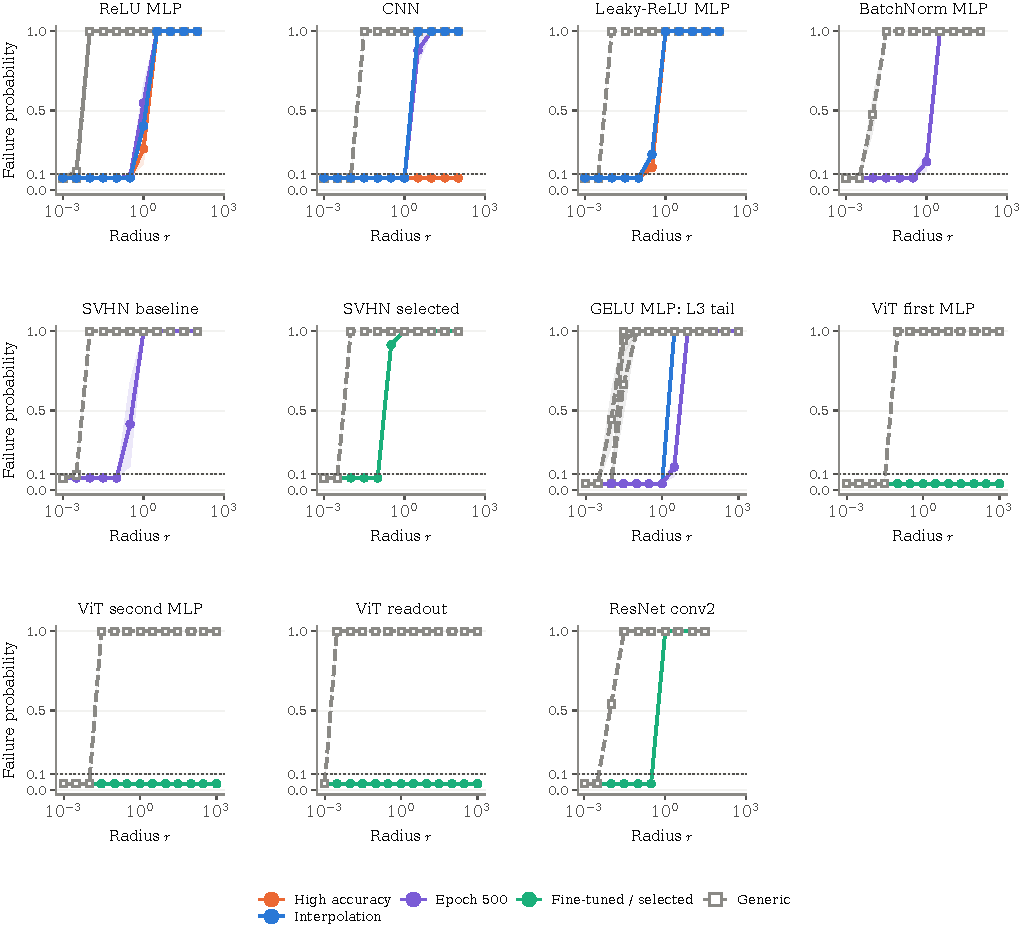
\includegraphics[width=6.149in]{radius_certificates.pdf}
\caption{Failure-probability upper bounds at absolute output tolerance $10^{-3}$. Solid curves: constructed spaces; dashed curves: generic controls. Colors denote training stages; shading is one sample SD across available seeds. The dotted line marks $10\%$ allowed failures. Bounds hold with $95\%$ simultaneous confidence over all 1126 comparisons in this figure; lines connect tested radii. GELU uses the approximate L3 kernel with $\sigma(J_3)/\sqrt{s}\le10^{-3}$. ViT shows first-MLP and readout feature-null edits and second-MLP downstream-null edits; ResNet shows the final convolution's selective family.}
\label{fig:radius-certificates-all}\label{fig:radius-variants}
\end{figure}
